% 原书 p.172–p.178（PDF p.180–p.186）
\chapter{杂论（Miscellaneous）}

% >>> p180
本章颇为特殊，宜视为前几章的补充。具体而言，它涵盖以下两个主要论题。其一，详述
第 5.4 节定理 5.4.1、第 6.3 节例 6.3.4 以及第 6.1 节定理 6.2.1 中的关键步骤。这些
关键步骤都基于同一种方法——Floer 延拓映射（Floer continuation map），它把不同
输入哈密顿函数所对应的哈密顿 Floer 同调群联系起来。其二，在一类特殊设定——环面
区域（toric domain）——上给出拉格朗日子流形的定量视角。环面区域族是第 2.5 节
定义 2.5.2 所引入辛环面流形的自然（且带几分「开放」意味的）推广。对环面区域而言，
其矩映射像提供了各种有用的定量信息，用以刻画辛刚性。特别地，与辛环面流形类似，
环面区域的纤维是分裂的拉格朗日环面，而这种分裂拉格朗日环面任一因子的尺寸，都启发
出对环面区域内嵌入拉格朗日环面的一个定量测度，称为形状不变量（shape invariant）。
事实证明，在某些情形下该量可以显式算出，从而给出一种新颖的「非线性」容量（参看
6.4 节定义 6.4.1），用来排除这类区域之间的嵌入。

\section{Floer 延拓映射（Floer Continuation Map）}

\begin{keytakeaways}
\begin{itemize}
  \item 几何图像：当哈密顿函数的输入量 $H$ 改变时，哈密顿 Floer 同调群之间并不
        是彼此无关的——存在一族由「同伦」$H_s$ 参数化的 $J$-全纯柱面，把 $H_1$
        的闭轨道「搬运」到 $H_2$ 的闭轨道，由此得到延拓映射。
  \item 核心工具：曲率带扰动的 $J$-全纯曲线方程 (7.4)、模空间计数 (7.2)、以及
        由模空间紧化边界（式 (7.6) 之前的分解）导出的链映射性质
        $\partial_{H_2}\circ\Phi=\Phi\circ\partial_{H_1}$。
  \item 关键定理：事实 7.1.1（不同同伦给出的链映射彼此链同伦），它保证延拓映射
        在同调层面良定义且与同伦、截断函数的选取无关。
  \item 定量结论：命题 7.1.1 给出延拓映射对作用量泛函的偏移控制 (7.6)、(7.7)，
        从而把过滤结构整体平移——这正是练习 7.1.1 中交换图与注 7.1.3 中
        「交错」的来源。
\end{itemize}
\end{keytakeaways}

本节中我们假定所讨论的辛流形 $(M,\omega)$ 是辛非球面的，即满足条件 (5.16)。给定
一个非退化哈密顿函数 $H\colon[0,1]\times M\to\R$（按定义 5.4.1 的意义）以及
$(M,\omega)$ 上一个通有的近复结构 $J$，按照 5.4 节所详述的构造，可以得到一个基于
哈密顿同痕 $\{\varphi_H^t\}_{t\in[0,1]}$ 的闭哈密顿轨道的同调理论，称为\textbf{
哈密顿 Floer 同调}，记作 $\mathrm{HF}_*(M,\omega,H,J)$，系数取在 $\Z_2$ 中。就
记号而言，它同时依赖 $H$ 与 $J$；而定理 5.4.1 确认：它其实是一个拓扑不变量
（与 $H$、$J$ 无关），并且还原出底辛流形 $(M,\omega)$ 的同调。这导致 5.3 节中
所展示的各种出人意料的刚性。

% >>> p181
若换一个更精细的视角：一旦把 $\mathrm{HF}_*(M,\omega,H,J)$ 升级为持续
$\Z_2$-模 $\mathbb{V}_H$（见 (6.2)），那么问题 6.2.1 问的就是：当输入哈密顿函数
由 $H$ 变为 $G$ 时，$\mathbb{V}_H$ 与 $\mathbb{V}_G$ 之间有何关系。定理 6.2.1 已
用条形码的语言回答了这一问题。

定理 5.4.1 与定理 6.2.1 的证明方式，都是在两个哈密顿 Floer 同调群之间直接构造一个
$\Z_2$-线性映射。为简洁起见，下文中把 $\mathrm{HF}_*(M,\omega,H,J)$ 记作
$\mathrm{HF}_*(H)$（相应的 Floer 链复形记作 $(\mathrm{CF}_*(H),\partial_H)$）。
对两个哈密顿函数 $H_1$ 与 $H_2$，我们想要构造下述映射
\begin{equation}\tag{7.1}
  \sigma_{H_1,H_2}\colon \mathrm{HF}_*(H_1)\to \mathrm{HF}_*(H_2),
\end{equation}
称之为 \textbf{Floer 延拓映射}。该映射保持次数（分次），但未必保持 (6.2) 中所定义
的作用量过滤。

与定义在同调群上的任何其他映射一样，人们首先需要在链复形上构造一个链映射（即与
边界映射交换的映射），也就是 $\Phi_{H_1,H_2}\colon \mathrm{CF}_*(H_1)\to
\mathrm{CF}_*(H_2)$。具体地，它定义如下：
\begin{equation}\tag{7.2}
  \Phi_{H_1,H_2}(x):=\sum_{\ind(x)=\ind(y)}\#_{\Z_2}\mathcal{M}(x,y)\,y,
\end{equation}
其中 $x$ 是一个闭哈密顿轨道，作为 $\mathrm{CF}_*(H_1)$ 的生成元；$y$ 是一个闭
哈密顿轨道，作为 $\mathrm{CF}_*(H_2)$ 的生成元。与 (5.23) 中 Floer 边界映射的
定义类似，$\mathcal{M}(x,y)$ 表示一个模空间，它由连接 $x$ 与 $y$ 的
$J$-全纯柱面组成，其连接方式将在下一段中详述。

取定一个截断函数 $\beta\colon\R\to[0,1]$，使它在 $s\le 1$ 时 $\beta(s)=0$、在
$s\ge 2$ 时 $\beta(s)=1$，并且是单调递增的。图 7.1 画出了这样一个函数的例子。

\begin{figure}[htbp]
  \centering
  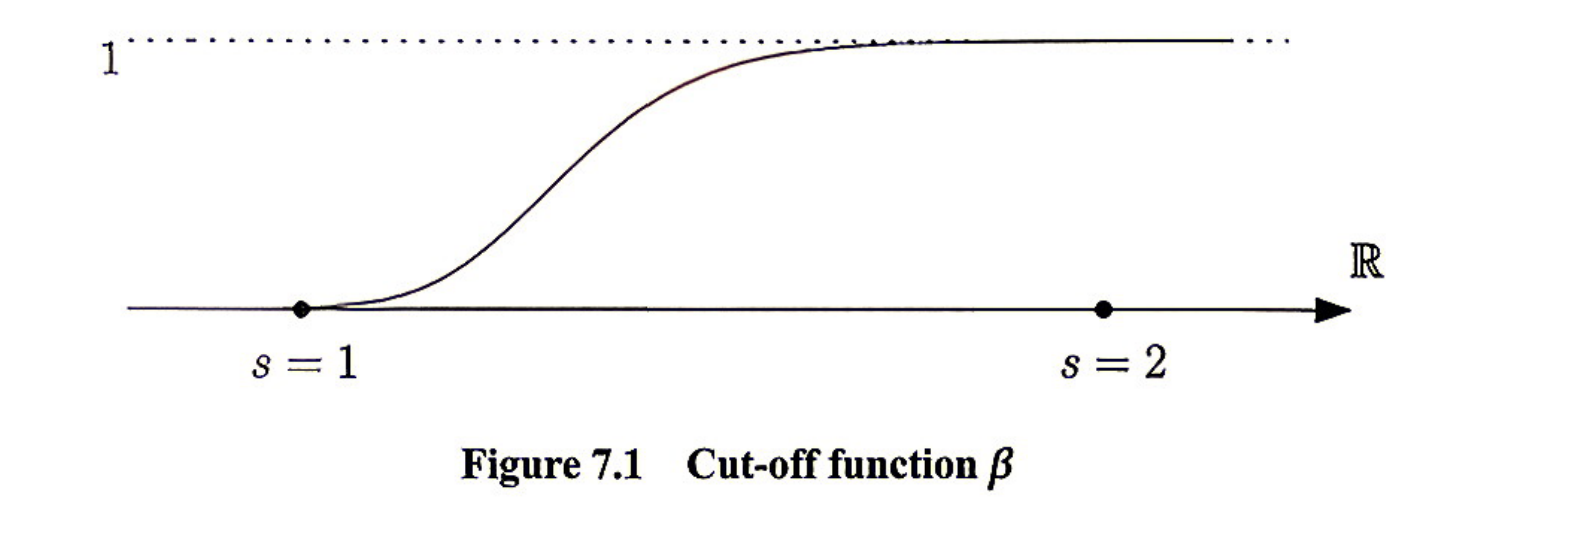
\includegraphics[width=0.72\linewidth]{figures/fig_p181_1.png}
  \caption*{图 7.1\quad 截断函数 $\beta$（原书 p.173, Figure 7.1；PDF p.181）}
\end{figure}

接着考虑由 $H_1$ 与 $H_2$ 的 $\beta(s)$-参数化组合所定义的线性同伦
$\mathcal{H}:=\{H_s\colon[0,1]\times M\to\R\}_{s\in\R}$，即
\begin{equation}\tag{7.3}
  H_s(t,p):=H_1(t,p)+\beta(s)\bigl(H_2(t,p)-H_1(t,p)\bigr).
\end{equation}
这一族（以 $s$ 为参数）哈密顿函数的同伦生成一族 $s$-族哈密顿向量场
$\{X_{H_s}\}_{s\in\R}$。与定义 Floer 边界映射时的 $J$-全纯曲线方程 (5.21) 不同，
这里我们考虑的 $J$-全纯曲线方程中，来自哈密顿向量场 $X_{H_s}$ 的扰动项也以 $s$
为参数，也就是说，考虑映射 $u\colon\R\times S^1\to M$ 满足
\begin{equation}\tag{7.4}
  \frac{\partial u}{\partial s}
  +J\bigl(u(s,t)\bigr)\left(\frac{\partial u}{\partial t}
  -X_{H_s}\bigl(u(s,t)\bigr)\right)=0.
\end{equation}

% >>> p182
于是模空间 $\mathcal{M}(x,y)$ 定义为
\[
  \mathcal{M}(x,y):=
  \left\{u\colon\R\times S^1\to M\ \middle|\
  \begin{array}{l}
    \dfrac{\partial u}{\partial s}
    +J\bigl(u(s,t)\bigr)\left(\dfrac{\partial u}{\partial t}
    -X_{H_s}\bigl(u(s,t)\bigr)\right)=0\\[6pt]
    \displaystyle\lim_{s\to-\infty}u(s,t)=x(t)\quad\text{且}\quad
    \lim_{s\to+\infty}u(s,t)=y(t)
  \end{array}\right\}.
\]
重要的是，这里满足 (7.4) 的曲线 $u$ \emph{不}容许 $\R$-作用（即在 $s$ 分量上的
平移），因为一般来说 $X_{H_{s+\tau}}\ne X_{H_s}$。于是 $\mathcal{M}(x,y)$ 的维数
（对通有的 $J$，此时它带有定义 5.1.2 中的带角流形结构）等于
$\ind(x)-\ind(y)$。由我们对 $y$ 的选取，模空间 $\mathcal{M}(x,y)$ 是紧的，且维数
为零，因此它是有限多个点的集合。

% [Tutor Note: 易错预警——(7.4) 中扰动项 $X_{H_s}$ 显式依赖 $s$，故模空间
% $\mathcal{M}(x,y)$ 没有平移不变性；其预期维数是 $\ind(x)-\ind(y)$，而不是
% Floer 边界映射模空间（方程 (5.21)) 的 $\ind(x)-\ind(y)-1$。差一个 $-1$ 的原因
% 正是 (5.21) 中的 $\R$-平移作用。核对 (7.2) 时请特别注意：求和只对
% $\ind(x)=\ind(y)$ 的 $y$ 进行，这正对应零维模空间。]

下一步，我们需要确认 $\Phi_{H_1,H_2}$（为简洁起见记作 $\Phi$）下降到同调层面，即
$\partial_{H_2}\circ\Phi=\Phi\circ\partial_{H_1}$。关键观察如下：对两个可缩的闭
哈密顿轨道 $x\in\Crit(\mathcal{A}_{H_1})$ 与 $z\in\Crit(\mathcal{A}_{H_2})$，
若 $\ind(x)-\ind(z)=1$，则相应的模空间 $\mathcal{M}(x,z)$（计数满足 (7.4) 的
$J$-全纯曲线）是带角流形，其紧化的边界分裂为以下几块（参看例 5.1.9）：
\[
  \partial\overline{\mathcal{M}}(x,z)
  =\left(\bigcup_{y\in\Crit(\mathcal{A}_{H_2})}
    \mathcal{M}(x,y)\times\mathcal{M}(y,z)\right)
  \cup\left(\bigcup_{w\in\Crit(\mathcal{A}_{H_1})}
    \mathcal{M}(x,w)\times\mathcal{M}(w,z)\right),
\]
其中右端恰好计数了那些对应于复合 $\partial_{H_2}\circ\Phi$ 与
$\Phi\circ\partial_{H_1}$ 的曲线。参见下面的示意图。

\begin{figure}[htbp]
  \centering
  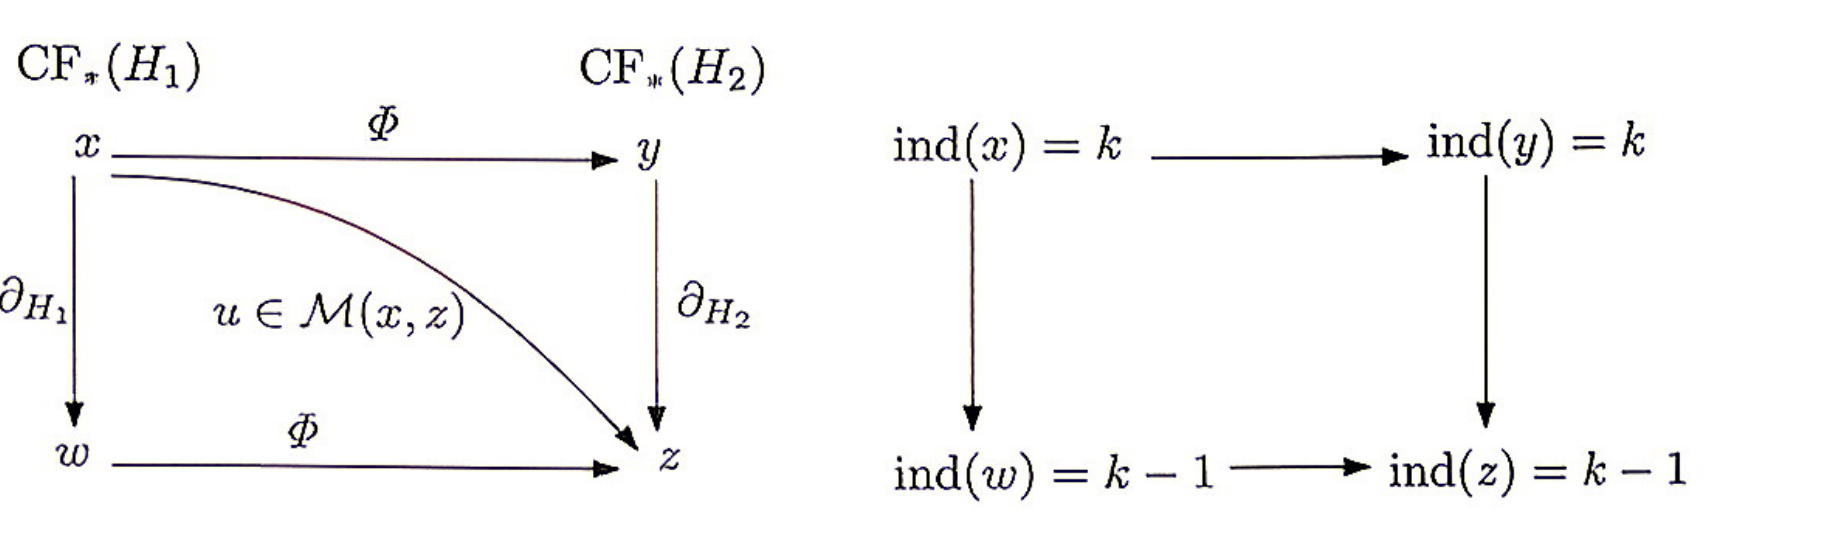
\includegraphics[width=0.78\linewidth]{figures/fig_p182_1.png}
  \caption*{示意图：链映射 $\Phi$ 与边界算子 $\partial_{H_1}$、$\partial_{H_2}$
    的交换关系及指标关系（原书 p.174 示意图，无编号；PDF p.182）}
\end{figure}

此外，$\#_{\Z_2}\partial\overline{\mathcal{M}}(x,z)=0$，因为
$\partial\overline{\mathcal{M}}(x,z)$ 是紧的一维流形。因此，(7.1) 中同调层面上的
Floer 延拓映射定义为 $\sigma_{H_1,H_2}:=(\Phi_{H_1,H_2})_*$。

% >>> p183
上面所定义的 $\Phi_{H_1,H_2}$，在链复形层面上似乎依赖于同伦
$\mathcal{H}=\{H_s\}_{s\in\R}$ 的选取（而后者又依赖于截断函数 $\beta$ 的选取）。
事实上，确实如此！下述事实展示了一个众所周知的结果，其证明是「模空间计数」方法
（正如在 (5.23) 与 (7.1) 中那样）的又一优美应用。

\whead{事实}{7.1.1$^{[222]}$}设 $(M,\omega)$ 是闭的辛非球面辛流形，$H_1,H_2$ 是
两个非退化哈密顿函数。则给定连接 $H_1$ 与 $H_2$ 的两个不同哈密顿函数同伦
$\mathcal{H}$ 与 $\mathcal{H}'$，它们诱导的链映射
$\Phi^{\mathcal{H}}_{H_1,H_2},\Phi^{\mathcal{H}'}_{H_1,H_2}\colon
\mathrm{CF}_*(H_1)\to\mathrm{CF}_*(H_2)$ 满足下述链同伦关系：
\[
  \Phi^{\mathcal{H}}_{H_1,H_2}-\Phi^{\mathcal{H}'}_{H_1,H_2}
  =K\circ\partial_{H_1}+\partial_{H_2}\circ K,
\]
其中 $K\colon\mathrm{CF}_*(H_1)\to\mathrm{CF}_{*+1}(H_2)$ 为某个映射。

% [Tutor Note: 含糊点拨——事实 7.1.1 的链同伦 $K$ 需由「在 $s$ 方向拼接两个同伦」
% 所得到的模空间计数显式给出；其紧化边界除两端外还出现第三类断裂曲线，正是这一项
% 贡献出 $K$。作者未展开之处在于：需要横截性（通有 $J$ 与通有同伦）保证模空间为
% 带角流形，以及需要能量估计/紧性（辛非球面条件排除了球面冒泡）。这是 Floer 原文
% （Floer, \emph{Symplectic fixed points and holomorphic spheres}, 1989）与
% McDuff--Salamon 教科书中关于延拓映射的标准论证。另请核对：$K$ 升一次指标，故
% $K\circ\partial_{H_1}$ 与 $\partial_{H_2}\circ K$ 的次数一致。]

注意，这一关系保证下降后的映射 $(\Phi^{\mathcal{H}}_{H_1,H_2})_*$ 与
$(\Phi^{\mathcal{H}'}_{H_1,H_2})_*$ 在哈密顿 Floer 同调群上相同。因此，在同构意义
下，诱导映射 $(\Phi_{H_1,H_2})_*$ 与连接 $H_1$、$H_2$ 的同伦选取无关。

\begin{wexam}{7.1.1}
  在闭的辛非球面辛流形 $(M,\omega)$ 上，事实 7.1.1 的一个特殊情形是 $H_1=H_2=H$。
  此时任何把 $H$ 与自身连接起来的同伦 $\mathcal{H}$ 都诱导一个「收缩」，即
  \[
    \Phi^{\mathcal{H}}_{H,H}-\mathbf{1}
    =K\circ\partial_H+\partial_H\circ K
  \]
  其中 $K\colon\mathrm{CF}_*(H)\to\mathrm{CF}_{*+1}(H)$ 为某个映射。为证明定理 5.4.1，
  我们可以如下「摆弄」同伦。考虑从 $H$ 到 $H'$ 的同伦 $\mathcal{H}$ 以及从 $H'$
  回到 $H$ 的同伦 $\mathcal{H}'$，则诱导的链映射满足：$\Phi^{\mathcal{H}'}_{H',H}
  \circ\Phi^{\mathcal{H}}_{H,H'}$ 收缩到恒等映射 $\mathbf{1}_{\mathrm{CF}_*(H)}$。
  再交换 $H$ 与 $H'$ 作对称论证，便得到：在同一个近复结构 $J$ 下，
  $\mathrm{HF}_*(M,\omega,H,J)\cong\mathrm{HF}_*(M,\omega,H',J)$。关于近复结构
  选取的无关性也可用同样方式得到。\hfill$//$
\end{wexam}

\begin{wrem}{7.1.1}
  若按 (7.1) 以完全严格的方式写下 Floer 延拓映射 $\sigma_{H_1,H_2}$，那么事实上
  $\mathrm{HF}_*(H_1)$ 与 $\mathrm{HF}_*(H_2)$ 之间并不存在「典范的」Floer
  延拓映射——总要先验地选取一份同伦数据 $\mathcal{H}$；而事实 7.1.1 只是说，两份
  这样的数据诱导出同一个同构（作为 $\Z_2$-模之间的 $\Z_2$-线性映射）。若要把这样
  的同伦数据编码进 Floer 延拓映射 $\sigma_{H_1,H_2}$，可以诉诸一种范畴式的描述，
  称为\textbf{连通简单系统}（connected simple system，见 [192]）。
\end{wrem}

为更直接地回答问题 6.2.1，人们或许会问：Floer 延拓映射 $\sigma_{H_1,H_2}$ 如何
改变过滤的哈密顿 Floer 同调？具体地说，对 Floer 链复形
$(\mathrm{CF}_*(H_1),\partial_{H_1})$ 与 $(\mathrm{CF}_*(H_2),\partial_{H_2})$，
分别按 (5.17) 定义辛作用量泛函 $\mathcal{A}_{H_1}$ 与 $\mathcal{A}_{H_2}$。若
$x$ 作为 $\mathrm{CF}_*(H_1)$ 的生成元、$y$ 作为 $\mathrm{CF}_*(H_2)$ 的生成元

% >>> p184
由 (7.2) 中的链映射 $\Phi_{H_1,H_2}$ 相联系，那么 $\mathcal{A}_{H_1}(x)$ 与
$\mathcal{A}_{H_2}(y)$ 之间有何关系？

与 6.3 节断言 6.3.1 中的论证类似，在同一个 Floer 链复形内部，若 $x,y$ 都是闭
哈密顿轨道且由 Floer 边界映射相连，则可验证
\begin{equation}\tag{7.5}
  \mathcal{A}_H(x)-\mathcal{A}_H(y)=E(u)\ge 0
\end{equation}
对任何满足 (5.21) 的连接柱面成立。这里 $E(u)$ 表示柱面 $u$ 的能量，如断言 6.3.1
的证明中那样。然而，当（带扰动的）$J$-全纯方程由 (5.21) 变为 (7.4) 时，除能量项
$E(u)$ 之外，还会出现某些额外的项。

\begin{wprop}{7.1.1}
  设 $x$ 是 $\{\varphi_{H_1}^t\}_{t\in[0,1]}$ 的一个闭哈密顿轨道，$y$ 是
  $\{\varphi_{H_2}^t\}_{t\in[0,1]}$ 的一个闭哈密顿轨道。选取 $x$ 的一个界定圆盘
  $w$。则对任何连接 $x$ 与 $y$、且关于某族哈密顿函数同伦
  $\{H_s\}_{s\in\R}$ 满足 (7.4) 的柱面 $u\colon\R\times S^1\to M$，对（$y$ 的）
  界定圆盘 $w\#u$，辛作用量泛函之间有下述关系：
  \begin{equation}\tag{7.6}
    \mathcal{A}_{H_1}\bigl((x,w)\bigr)-\mathcal{A}_{H_2}\bigl((y,w\#u)\bigr)
    =E(u)-\int_{-\infty}^{\infty}\!\!\int_0^1
    \frac{\partial H_s}{\partial s}\bigl(t,u(s,t)\bigr)\,\dd t\,\dd s.
  \end{equation}
  特别地，若 $\{H_s\}_{s\in\R}$ 是 (7.3) 中的线性同伦，则我们有
  \begin{equation}\tag{7.7}
    \mathcal{A}_{H_2}\bigl((y,w\#u)\bigr)-\mathcal{A}_{H_1}\bigl((x,w)\bigr)
    \le\int_0^1\max_M\bigl(H_2(t,\cdot)-H_1(t,\cdot)\bigr)\,\dd t.
  \end{equation}
\end{wprop}

\begin{wproof}
  在 (7.6) 成立的前提下，由我们对 $H_s$ 的选取可知
  \begin{align*}
    \int_{-\infty}^{\infty}\!\!\int_0^1
    \frac{\partial H_s}{\partial s}\bigl(t,u(s,t)\bigr)\,\dd t\,\dd s
    &=\int_{-\infty}^{\infty}\!\!\int_0^1
      \beta'(s)(H_2-H_1)\bigl(t,u(s,t)\bigr)\,\dd t\,\dd s\\
    &\le\left(\int_0^1\max_M\bigl(H_2(t,\cdot)-H_1(t,\cdot)\bigr)\,\dd t\right)
      \left(\int_{-\infty}^{\infty}\beta'(s)\,\dd s\right)\\
    &=\int_0^1\max_M\bigl(H_2(t,\cdot)-H_1(t,\cdot)\bigr)\,\dd t,
  \end{align*}
  因为 $\int_{-\infty}^{\infty}\beta'(s)\,\dd s=1$。回到 (7.6)，
  \begin{align*}
    \text{(7.6) 的左端}
    &=-\int_{-\infty}^{\infty}\frac{\dd}{\dd s}
      \mathcal{A}_H\bigl(w\#u(s,t)\bigr)\,\dd s\\
    &=\int_{-\infty}^{\infty}\frac{\dd}{\dd s}\left(
      \int_{D^2}\bigl(w\#u(s,t)\bigr)^*\omega
      -\int_0^1 H_s\bigl(t,u(s,t)\bigr)\,\dd t\right)\dd s\\
    &=\int_{-\infty}^{\infty}\!\!\int_0^1
      \omega\left(\frac{\partial u}{\partial s},\frac{\partial u}{\partial t}\right)
      \dd t\,\dd s
      -\int_{-\infty}^{\infty}\!\!\int_0^1\left(
      \frac{\partial H_s}{\partial s}
      +\omega\left(\frac{\partial u}{\partial s},X_{H_s}\right)\right)\dd t\,\dd s\\
    &=\int_{-\infty}^{\infty}\!\!\int_0^1\left(
      -\frac{\partial H_s}{\partial s}
      +\omega\left(\frac{\partial u}{\partial s},
      \frac{\partial u}{\partial t}-X_{H_s}\right)\right)\dd t\,\dd s\\
    &=E(u)-\int_{-\infty}^{\infty}\!\!\int_0^1
       \frac{\partial H_s}{\partial s}\bigl(t,u(s,t)\bigr)\,\dd t\,\dd s
      =\text{(7.6) 的右端}.
  \end{align*}
% >>> p185
  这就完成了证明。
\end{wproof}

% [Tutor Note: 易错预警——(7.6) 与 (7.7) 的符号方向是本段最容易出错之处。(7.6)
% 左端是 $\mathcal{A}_{H_1}-\mathcal{A}_{H_2}$，与通常的「能量非负」方向相反；
% 只有把同伦导数项移到另一边才得到 (7.7)。当 $H_1\ge H_2$ 逐点成立时
% $\max_M(H_2-H_1)\le 0$，于是 $\mathcal{A}_{H_2}\le\mathcal{A}_{H_1}<\lambda$，
% 过滤才被保持（见下文 (7.8) 的过滤移位方向）。另注意此处 $\partial H_s/\partial s$
% 的一项来自 $H_s$ 对 $s$ 的显式依赖，而非对 $(t,u)$ 的全微分。]

\begin{wrem}{7.1.2}
  请注意，(7.6) 中与 (7.5) 相比多出的那一项，来自对 $H_s(t,u(s,t))$ 关于 $s$
  求导。
\end{wrem}

对任意 $\lambda\in\R$，以 $\mathrm{CF}_*^{\lambda}(H)$ 表示
$(\mathrm{CF}_*(H),\partial_H)$ 中由作用量 $\mathcal{A}_H(x)<\lambda$ 的闭哈密顿
轨道 $x$ 所生成的那个子复形。于是命题 7.1.1 表明
\[
  \Phi_{H_1,H_2}\colon\mathrm{CF}_*^{\lambda}(H_1)
  \to\mathrm{CF}_*^{\lambda+\int_0^1\max_M(H_2(t,\cdot)-H_1(t,\cdot))\,\dd t}(H_2),
\]
即过滤发生了平移。同调群上诱导的 Floer 延拓映射满足
\begin{equation}\tag{7.8}
  \sigma_{H_1,H_2}\colon
  H_*\bigl(\mathrm{CF}^{\lambda}(H_1),\partial_{H_1}\bigr)
  \to H_*\Bigl(\mathrm{CF}^{\lambda+\int_0^1
  \max_M(H_2(t,\cdot)-H_1(t,\cdot))\,\dd t}(H_2),\partial_{H_2}\Bigr).
\end{equation}
沿用 (6.2) 的记号，我们有
$\sigma_{H_1,H_2}\colon V_{H_1,\lambda}\to
V_{H_2,\lambda+\int_0^1\max_M(H_2(t,\cdot)-H_1(t,\cdot))\,\dd t}$。

\begin{wexer}{7.1.1}
  沿用上述讨论中的记号，对任意 $\lambda\in\R$，下述图表交换：

  \begin{figure}[htbp]
    \centering
    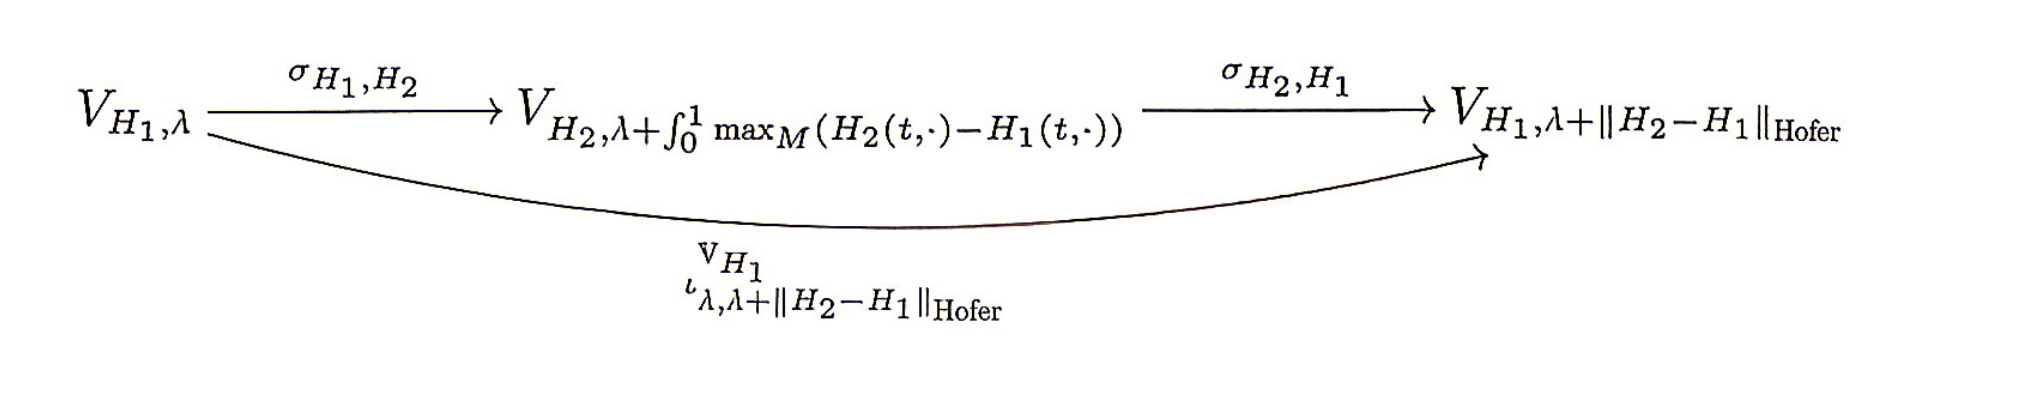
\includegraphics[width=0.8\linewidth]{figures/fig_p185_2.png}
    \caption*{练习 7.1.1 的交换图（其一）：经
      $\sigma_{H_1,H_2}$ 与 $\sigma_{H_2,H_1}$ 的复合
      （原书 p.177 示意图，无编号；PDF p.185）}
  \end{figure}

  \begin{figure}[htbp]
    \centering
    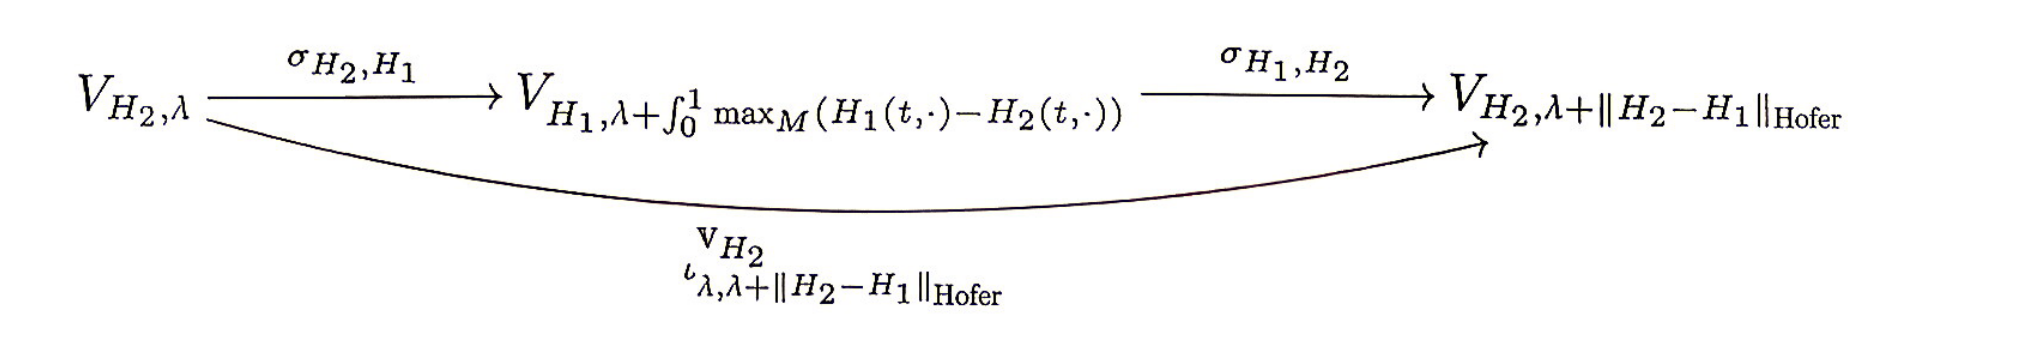
\includegraphics[width=0.8\linewidth]{figures/fig_p185_3.png}
    \caption*{练习 7.1.1 的交换图（其二）：交换 $H_1$ 与 $H_2$ 后的对应图表
      （原书 p.177 示意图，无编号；PDF p.185）}
  \end{figure}

  其中 $\|H_2-H_1\|_{\mathrm{Hofer}}$ 表示哈密顿函数 $H_2-H_1$ 的 Hofer 范数
  （如 (6.1) 中那样），而 $\iota_{\cdot,\cdot}$ 表示由过滤链复形的包含所诱导的
  映射。
\end{wexer}

\begin{wrem}{7.1.3}
  用持续模的语言来说，练习 7.1.1 证明了持续模 $\mathbb{V}_{H_1}$ 与
  $\mathbb{V}_{H_2}$ 是 $\|H_2-H_1\|_{\mathrm{Hofer}}$-交错的（见第 4 章、
  [45] 中的 5.1 节以及 [44] 中的定义 4.2）。最终这将推出定理 6.2.1 的结论。
\end{wrem}

本节最后，让我们重新审视例 6.3.4 以及定义 6.3.1（$\C^n$ 中区域的辛同调）。在那里
需要有一个定义良好的、保持过滤的 Floer 延拓映射
$\sigma_{H_1,H_2}\colon\mathrm{HF}_*^{(\lambda,\infty)}
(\C^n,\dd\lambda_{\mathrm{std}},H_1,J)\to\mathrm{HF}_*^{(\lambda,\infty)}
(\C^n,\dd\lambda_{\mathrm{std}},H_2,J)$。按定义，可以如下等同：
\[
  \mathrm{HF}_*^{(\lambda,\infty)}(\C^n,\dd\lambda_{\mathrm{std}},H_1,J)
  \cong\mathrm{HF}_*(\C^n,\dd\lambda_{\mathrm{std}},H_1,J)
  \big/\mathrm{HF}_*^{\lambda}(\C^n,\dd\lambda_{\mathrm{std}},H_1,J),
\]

% >>> p186
这与 $\mathrm{HF}_*^{(\lambda,\infty)}(\C^n,\dd\lambda_{\mathrm{std}},H_2,J)$
类似。因此，若在 $[0,1]\times M$ 上逐点有 $H_1\ge H_2$ 且
$\mathcal{A}_{H_1}((x,w))<\lambda$，则命题 7.1.1 中的 (7.7) 适用，我们得到
\begin{align*}
  \mathcal{A}_{H_2}\bigl((y,w\#u)\bigr)
  &\le\mathcal{A}_{H_1}\bigl((x,w)\bigr)
    +\int_0^1\max_M\bigl(H_2(t,\cdot)-H_1(t,\cdot)\bigr)\,\dd t\\
  &\le\mathcal{A}_{H_1}\bigl((x,w)\bigr)<\lambda.
\end{align*}
注意，这一关于哈密顿函数的单调性条件恰是 (6.17) 中给出的条件。更重要的是，当
交换 $H_1$ 与 $H_2$ 的角色时，$\sigma_{H_2,H_1}$ 可能并非良定义；因此，与例
7.1.1 末尾所详述的闭流形情形不同，我们不能直接断言 $\sigma_{H_1,H_2}$（或
$\sigma_{H_2,H_1}$）是同构。事实上，我们在例 6.3.5 中已经见过这些 Floer 延拓映射
给出的非同构。这本质上区分了应用于闭辛流形的 Floer 同调与应用于（开）刘维尔
流形中的刘维尔区域的 Floer 同调。

% [Tutor Note: 原文疑误——本段末句原文作 "the Floer homology applied to a
% Liouville domains in (an open) Liouville manifold"，其中 "a ... domains" 数
% 不一致（应为 a Liouville domain 或 Liouville domains）。译文按语义处理为
% 「刘维尔区域」，不影响数学内容；已记入审校记录。另请注意：闭流形情形之所以能
% 用「$H\to H'$ 再 $H'\to H$」证明同构，关键在于两侧延拓映射都良定义；开流形上
% 过滤迫使只能单向比较，这正是持续模而非同构的来源。]
